\documentclass[spanish, c]{beamer}

\usepackage[utf8]{inputenc}
% \usepackage[spanish, mexico]{babel}
\usepackage{amsmath}
\usepackage{mathtools}
\usepackage{hyperref}
\usepackage{xcolor}
\usepackage{color}
\usepackage{ragged2e}
\usepackage{mathrsfs}
% \usepackage{csquotes}
% \usepackage{listings}
\usepackage[scaled]{beramono}
\usepackage[T1]{fontenc}
\usepackage{graphicx}
\usepackage{booktabs}
\usepackage{physics}
\usepackage{minted}
\usepackage{tcolorbox}
\usepackage{tikz}
\usepackage{relsize}
\usepackage{algorithm}
\usepackage{algpseudocode}
\usepackage[shortlabels]{enumitem}
\usepackage{pifont}

\newcommand{\cmark}{\ding{51}}%
\newcommand{\xmark}{\ding{55}}%

\setlist[itemize]{label=\textbullet}  % global enumitem for default itemize

\tcbuselibrary{minted, skins}

\usetikzlibrary{arrows, automata, positioning, fit, shapes.geometric, backgrounds}
  
  \tikzset{
    stylename/.style={
      ->, %arrow type
      >=stealth', %arrow head type (bold)
      shorten >=1pt, 
      auto,
      %semithick,
      initial text=$ $, %no start text
    }
  }

\renewcommand{\indent}{\hspace*{2em}}

\newcommand\CC{C\nolinebreak[4]\hspace{-.05em}\raisebox{.4ex}{\relsize{-3}{\textbf{++}}}~}
\newcommand{\bigO}{\mathcal{O}}

\renewcommand{\Comment}[2][.55\linewidth]{%
  \leavevmode\hfill\makebox[#1][l]{\fontfamily{cmss}\selectfont\color{red}\footnotesize$\longrightarrow$\quad#2}}
% \usepackage{tikz}

% \usetikzlibrary{fit, shapes, arrows}

% \usepackage{courier}
% \usepackage{subfigure}
% \usepackage{enumerate}
% \usepackage{algorithmic}
% \usepackage{algorithm}

% \usepackage{listings}
% \usepackage{lstlinebgrd}

\usetheme{Boadilla}
\usefonttheme[onlymath]{serif}

\newcommand\blfootnote[1]{%
\begingroup
\renewcommand\thefootnote{}\footnote{#1}%
\addtocounter{footnote}{-1}%
\endgroup
}

\algrenewcommand\alglinenumber[1]{\footnotesize #1}

\makeatletter
% start with some helper code
% This is the vertical rule that is inserted
\newcommand*{\algrule}[1][\algorithmicindent]{%
  \makebox[#1][l]{%
    \hspace*{.2em}% <------------- This is where the rule starts from
    \vrule height .75\baselineskip depth .25\baselineskip
  }
}

\newcount\ALG@printindent@tempcnta
\def\ALG@printindent{%
    \ifnum \theALG@nested>0% is there anything to print
    \ifx\ALG@text\ALG@x@notext% is this an end group without any text?
    % do nothing
    \else
    \unskip
    % draw a rule for each indent level
    \ALG@printindent@tempcnta=1
    \loop
    \algrule[\csname ALG@ind@\the\ALG@printindent@tempcnta\endcsname]%
    \advance \ALG@printindent@tempcnta 1
    \ifnum \ALG@printindent@tempcnta<\numexpr\theALG@nested+1\relax
    \repeat
    \fi
    \fi
}
% the following line injects our new indent handling code in place of the default spacing
\patchcmd{\ALG@doentity}{\noindent\hskip\ALG@tlm}{\ALG@printindent}{}{\errmessage{failed to patch}}
\patchcmd{\ALG@doentity}{\item[]\nointerlineskip}{}{}{} % no spurious vertical space
% end vertical rule patch for algorithmicx
\makeatother
%

% Sets the templates
\definecolor{navyblue}{RGB}{0, 0, 128}
\definecolor{crimson}{RGB}{128, 16, 0}

\setbeamertemplate{navigation symbols}{}
\setbeamertemplate{headline}{}
\setbeamertemplate{title page}[default][colsep=-4bp,rounded=true]
\setbeamertemplate{footline}[frame number]
\setbeamertemplate{bibliography item}[text]
\setbeamertemplate{theorems}[numbered]

\setbeamercolor{title}{fg=navyblue, bg=white}
\setbeamercolor{frametitle}{fg=navyblue, bg=white}
\setbeamercolor{structure}{fg=navyblue}
\setbeamercolor{button}{fg=white,bg=navyblue}

\setbeamercovered{transparent}

\tcbset{cppexample/.style={%
    colback=green!5,
    colframe=green!30!black,
    listing only,
    fonttitle=\bfseries,
    listing engine=minted,
    minted language=c++,
    enhanced,
    overlay={\begin{tcbclipinterior}\fill[red!25!green!25!white] (frame.south west)rectangle ([xshift=4mm]frame.north west);\end{tcbclipinterior}}
}}

\tcbset{cppfullexample/.style={%
    % colback=green!5,
    % colframe=green!30!black,
    listing only,
    fonttitle=\bfseries,
    listing engine=minted,
    minted language=c++,
    enhanced,
    overlay={\begin{tcbclipinterior}\fill[black!20!white] (frame.south west)rectangle ([xshift=4mm]frame.north west);\end{tcbclipinterior}}
}}

\tcbset{cppfullborderless/.style={%
    % colback=green!5,
    % colframe=green!30!black,
    listing only,
    listing engine=minted,
    minted language=c++,
    enhanced,
    overlay={\begin{tcbclipinterior}\fill[black!20!white] (frame.south west)rectangle ([xshift=4mm]frame.north west);\end{tcbclipinterior}}
}}

\title{Abstracción de Datos y Listas Encadenadas}
\subtitle{Programación de Estructuras de Datos y Algoritmos Fundamentales \\ (TC1031)}
\author{
    \texorpdfstring{
        \begin{center}
            M.C. Xavier Sánchez Díaz \\
            \href{mailto:sax@tec.mx}{\texttt{sax@tec.mx}}
        \end{center}
    }
    {M.C. Xavier Sánchez Díaz}
}

\institute[Tecnológico de Monterrey]{\includegraphics[scale=0.5]{../img/logo}}
\date{}

\begin{document}

\setlength{\rightskip}{0pt}

\begin{frame}[plain]
    \titlepage        
\end{frame}

\begin{frame}{Outline}
    \tableofcontents
\end{frame}

\section{Abstracción de Datos}

\begin{frame}{Tipos de datos}{Abstracción de Datos}
    A lo largo del curso hemos usado \alert{tipos de datos} (\textit{datatypes}) para nuestros vectores y arreglos. \pause
    
    \bigskip

    Estos \textbf{tipos de datos} han sido para representar los siguientes datos: \pause

    \bigskip

    \begin{itemize}
        \item \texttt{int} o números enteros
        \item \texttt{float} o números flotantes (decimales)
        \item \texttt{string} o cadenas de caracteres (`palabras')
    \end{itemize} \pause

    \bigskip

    Y cada uno de ellos tiene un \textit{operaciones válidas} y un \textit{rango} asociados.
\end{frame}

\begin{frame}{Datos más complicados}{Abstracción de datos}
    ¿Qué pasa si en lugar de números, quiero trabajar con \textit{otra cosa}? \pause

    \bigskip

    Por ejemplo, a una {\color<3->{blue}coordenada} en formato $(x,y)$ puedo \textit{sumarle} una magnitud y debería obtener \textit{otra} {\color<3->{blue}coordenada}. \pause

    \bigskip

    En este caso, las {\color{blue}{coordenadas}} son un \textit{dato estructurado}: \pause

    \begin{itemize}
        \item Tiene una $x$
        \item Tiene una $y$
        \item Tiene una representación textual en formato $(x,y)$
        \item Puedo sumarle (y restarle) magnitudes para obtener otras {\color{blue}{coordenadas}}
    \end{itemize} \pause

    \bigskip

    Ésta es una \alert{estructura de datos}.

\end{frame}

\begin{frame}[plain]
    \begin{center}
        \Huge
        \textit{Story time:} \texttt{structs} vs \texttt{objects} \pause

        \vspace{5ex}

        \textit{Story time: \texttt{Old Style} vs \texttt{New Style}}
    \end{center}
\end{frame}

\subsection{Diseñando Estructuras de Datos}

\begin{frame}{Niveles de abstracción de datos}

    \begin{description}[style=unboxed]
        \itemsep2.5ex
        \item [Abstracción.] Cuando organizamos los datos de alguna manera \alert{lógica} o \textit{abstracta}---general---que después pueda ser aterrizada a distintas implementaciones. El \textbf{`qué'} se explica en este nivel.
        \item [Implementación.] En este nivel se definen e \alert{implementan} las operaciones posibles que se le pueden aplicar a la estructura. El \textbf{`cómo'} se explica en este nivel.
        \item [Aplicación.] Se aterriza dicha estructura a un uso específico por medio de una \alert{instancia} y se utiliza para resolver el problema correspondiente. El \textbf{`dónde'} o \textbf{`con qué'} se explica en este nivel.
    \end{description}
\end{frame}

\begin{frame}{¿Qué tiene una estructura de datos \textit{Old Style}?}{Abstracción de Datos}

    \begin{itemize}
        \item Los {\color{red} \textbf{elementos}} de la estructura son parte del {\color{red} `qué'} \pause
        \item La {\color{red} \textbf{organización}} de los elementos de la estructura\pause
        \item El {\color{red} \textbf{dominio}} de los datos de la estructura \pause
        \item Las {\color{blue} \textbf{operaciones}} que pueden aplicarse a la estructura son parte del {\color{blue} cómo} \pause
    \end{itemize}

    \bigskip

    Ejemplo: una \textbf{matriz} tiene

    \begin{itemize}
        \item \textbf{Celdas} como {\color{red} \textbf{elementos}} \pause
        \item Se {\color{red} \textbf{organiza}} en \textbf{renglones} y \textbf{columnas} \pause
        \item Puede tener los {\color{red} \textbf{valores}} que nosotros determinemos \pause
        \item Se le pueden {\color{blue} sumar/restar/multiplicar} escalares o con otras matrices (bajo \textit{ciertas condiciones})
    \end{itemize}
\end{frame}

\begin{frame}[plain]
    \begin{center}
        \Huge
        Disclaimer 1: \textit{Todo es matemáticas. Esto no se limita a Ciencias Computacionales}

        \bigskip

        Disclaimer 2: \textit{Todo se hace ahora con objetos}\footnote{Estamos en el siglo XXI, come on\dots}
    \end{center}
\end{frame}

\section{Listas vinculadas (\textit{Linked lists})}

\begin{frame}{Listas vinculadas}
    Una \alert{lista vinculada} (\textit{linked list})---o simplemente \textit{lista}---es una estructura de datos \textbf{recursiva} que tiene una organización lineal (como la de un arreglo) y donde cada \textbf{nodo} tiene dos `celdas': una dirección (contenido) y un decremento (un apuntador a otra celda).

    \bigskip

    \begin{center}
        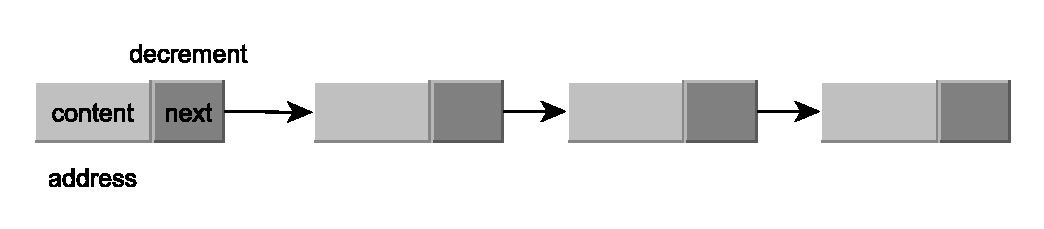
\includegraphics[width=0.95\textwidth]{list.pdf}
    \end{center} \pause

    \bigskip

    \begin{center}
        Story time: \texttt{CAR} vs. \texttt{CDR}
    \end{center}
\end{frame}

\section{Pilas (\textit{Stack})}

\begin{frame}{Pilas}
    Una \alert{pila} (\textit{stack}) es una estructura de datos de organización lineal (como la de un arreglo o una lista vinculada), en donde vamos \textbf{apilando} los elementos. Como un montón de platos apilados, el que sacas (a menos que estés demente) suele ser el de hasta arriba (que es el último que entró): FILO mode.

    \begin{center}
        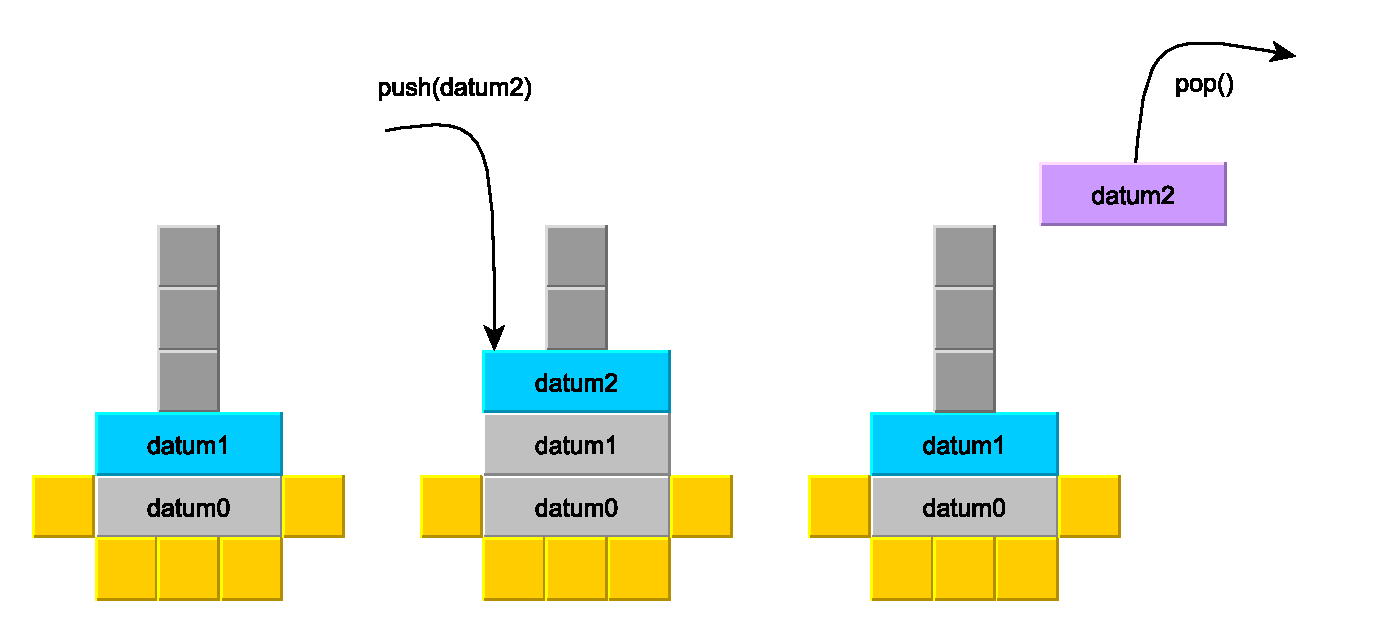
\includegraphics[width=0.75\textwidth]{stack.pdf}
    \end{center} \pause

    \begin{center}
        ¿A qué crees que se refiere el famoso \textit{Stack Overflow}?
    \end{center}

\end{frame}

\section{Colas (\textit{Queue})}

\begin{frame}{Colas}    
    Una \alert{cola} (\textit{queue}) es una estructura de datos de organización lineal (como la de un arreglo o una lista vinculada), en donde vamos \textbf{enfilando} los elementos. Como un montón de personas enfiladas, el que pasa primero (a menos que tenga paros) suele ser el que está hasta adelante (que es el primero que se formó): FIFO mode.
    \begin{center}
        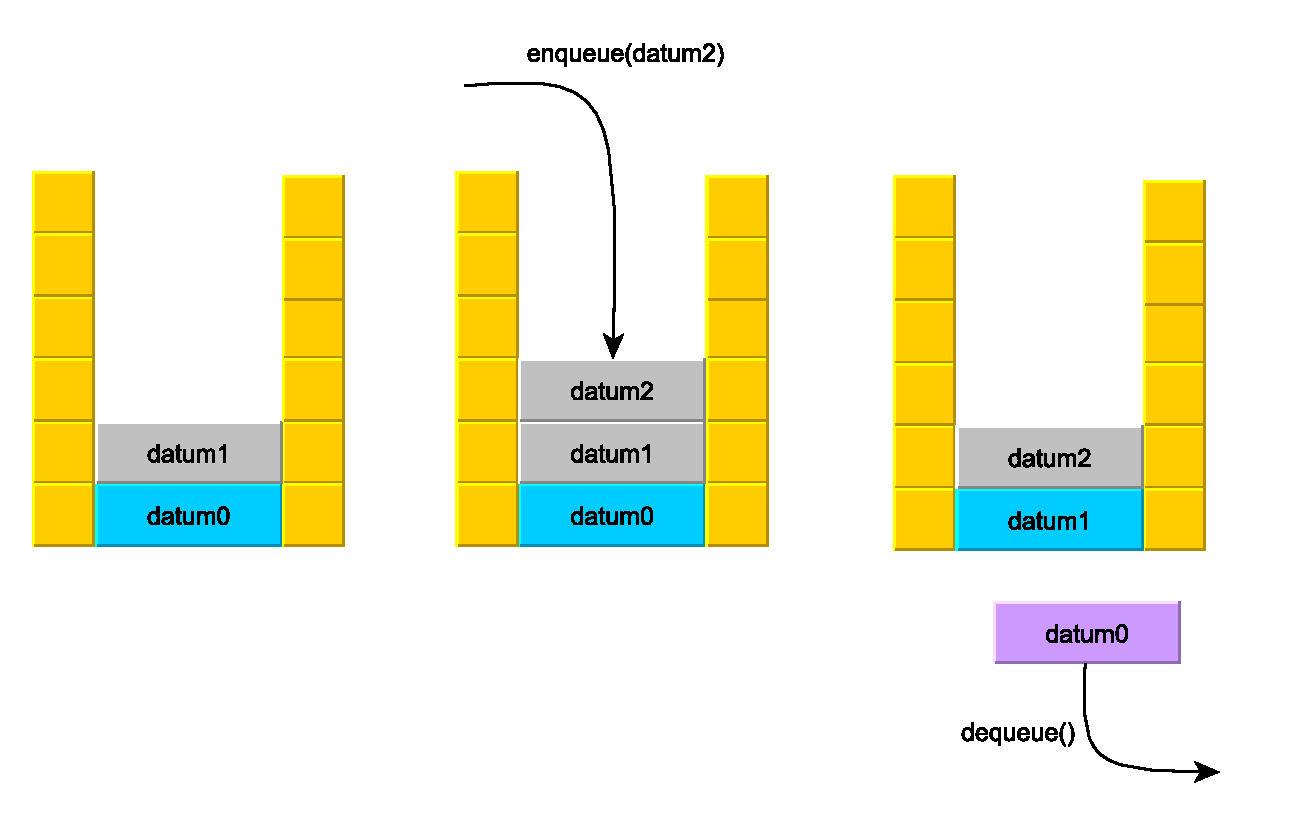
\includegraphics[width=0.69\textwidth]{queue.pdf}
    \end{center}
\end{frame}

\begin{frame}[plain]
    \begin{center}
        \Huge
        Quiz time!
    \end{center}
\end{frame}

\begin{frame}[plain]
    
    \begin{center}
        \includegraphics[width=0.6\textwidth]{creeper-queue.png}

        \bigskip

        {\huge Creeper stack or Creeper queue?}
    \end{center}

\end{frame}

\begin{frame}[plain]
    
    \begin{center}
        \includegraphics[width=0.55\textwidth]{soshi-pile.jpg}

        \bigskip

        {\huge SoShi stack or SoShi queue?}
    \end{center}

\end{frame}

\begin{frame}[plain]

    \begin{center}
        \texttt{sizeOf(mylist.push(mynumber + 5))}    

        \bigskip

    {\huge Function stack or function queue?}
    \end{center}

\end{frame}


\begin{frame}[plain]

    \begin{center}
        \texttt{mynumber = mynumber + 5;\\mylist.push(mynumber);\\mylist.getSize();}
        
        \bigskip

    {\huge Function stack or function queue?}
    \end{center}

\end{frame}



% \section*{Referencias}

% \begin{frame}[t]{Referencias}
    % \nocite{bibID01}
    % \nocite{bibID02}

    % \bibliographystyle{IEEE}
    % \bibliography{biblio}
% \end{frame}

\end{document}